% Created 2022-05-31 Tue 22:48
% Intended LaTeX compiler: pdflatex
\documentclass[
                        12pt, % Main document font size
                        a4paper, % Paper type, use 'letterpaper' for US Letter paper
                        oneside, % One page layout (no page indentation)
                        %twoside, % Two page layout (page indentation for binding and different headers)
                        headinclude,footinclude, % Extra spacing for the header and footer
                        BCOR5mm, % Binding correction
                  ]{scrartcl}
                  \usepackage[
                        nochapters, % Turn off chapters since this is an article
                        beramono, % Use the Bera Mono font for monospaced text (	exttt)
                        eulermath,% Use the Euler font for mathematics
                        pdfspacing, % Makes use of pdftex’ letter spacing capabilities via the microtype package
                        dottedtoc % Dotted lines leading to the page numbers in the table of contents
                  ]{classicthesis} % The layout is based on the Classic Thesis style
                  \usepackage{arsclassica} % Modifies the Classic Thesis package
                  \usepackage[T1]{fontenc} % Use 8-bit encoding that has 256 glyphs
                  \usepackage[utf8]{inputenc} % Required for including letters with accents
                  \usepackage{graphicx} % Required for including images
                  \usepackage{enumitem} % Required for manipulating the whitespace between and within lists
                  \usepackage{lipsum} % Used for inserting dummy 'Lorem ipsum' text into the template
                  \usepackage{subfig} % Required for creating figures with multiple parts (subfigures)
                  \usepackage{amsmath,amssymb,amsthm} % For including math equations, theorems, symbols, etc
                  \usepackage{qsharp} % qsharp minted highlighting
                  \usepackage{varioref} % More descriptive referencing
                  \usepackage{mdframed}
                  \BeforeBeginEnvironment{minted}{\begin{mdframed}}
                  \AfterEndEnvironment{minted}{\end{mdframed}}
\usepackage[utf8]{inputenc}
\usepackage[T1]{fontenc}
\usepackage{graphicx}
\usepackage{longtable}
\usepackage{wrapfig}
\usepackage{rotating}
\usepackage[normalem]{ulem}
\usepackage{amsmath}
\usepackage{amssymb}
\usepackage{capt-of}
\usepackage{hyperref}
\usepackage{minted}
\author{Daniel Biasiotto}
\date{\today}
\title{Calcolabilitá e Complessitá}
\hypersetup{
 pdfauthor={Daniel Biasiotto},
 pdftitle={Calcolabilitá e Complessitá},
 pdfkeywords={},
 pdfsubject={},
 pdfcreator={Emacs 28.1 (Org mode 9.6)}, 
 pdflang={English}}
\begin{document}

\maketitle
\tableofcontents

\begin{itemize}
\item Prof: Stefano Berardi
\item \href{./20210921121153-calcolabilita\_e\_complessita.pdf}{PDF Version}
\end{itemize}
\section{Info Corso}
\label{sec:orgd5c305c}
\begin{itemize}
\item Testo:
\begin{itemize}
\item \href{20210921121359-introduction_to_the_theory_of_computation.org}{Introduction to the theory of Computation}
\end{itemize}
\item Link:
\begin{itemize}
\item \url{https://turingmachinesimulator.com/}
\end{itemize}
\end{itemize}
\section{Teoria}
\label{sec:org8e24937}
\subsection{Macchina di Turing}
\label{sec:org7fd5678}
\uline{The Church-Turing Thesis}
Utilizzata per definire un problema risolvibile
\begin{itemize}
\item nato per dare una definizione semplice di risolvibilitá
\begin{itemize}
\item un qualsiasi computer puó essere ridefinito con una \texttt{MdT} equivalente
\end{itemize}
\item unico accesso alla memoria
\begin{itemize}
\item come un nastro, legge dall'inizio fino alla fine
\begin{itemize}
\item lenta
\item non é una architettura realmente implementabile
\end{itemize}
\end{itemize}
\end{itemize}

Caratterizzata da:
\begin{itemize}
\item controllo
\begin{itemize}
\item stati interni
\begin{itemize}
\item che definiscono comportamenti diversi
\end{itemize}
\end{itemize}
\item memoria/tape
\begin{itemize}
\item testa di lettura
\item alfabeto a scelta
\end{itemize}

\item l'Input é finito
\item la fine del Input é marcata con un simbolo speciale
\end{itemize}

A differenza degli Automi a Stati Finiti puó sovrascrivere, appunta per aiutarsi nell'esecuzione
\begin{itemize}
\item una macchina di turing puó simulare qualsiasi macchina a differenza di un DFA
\end{itemize}
La Macchina di Turing essendo estremamente semplice é ottima per lo studio della Calcolabilitá

\subsubsection{Definizione Formale}
\label{sec:org39af058}
\texttt{MT 1936}
7-tupla \((Q,\Sigma,\Gamma,\delta,q_0,q_{accept},q_{reject})\)
\begin{enumerate}
\item \(Q\): insieme di stati
\item \(\Sigma\): alfabeto di Input non contenente il simbolo di blank
\item \(\Gamma\): alfabeto del nastro
\item \(\delta: Q \times \Gamma \rightarrow Q \times \Gamma \times \{L,R\}\): funzione di transizione
\begin{itemize}
\item Left (<) / Right (>)
\end{itemize}
\item \(q_{accept}\)
\end{enumerate}


\begin{itemize}
\item Lo stato di rifiuto non viene inserito, é sottointeso a ogni Input non riconosciuto una transizione allo stato di rifiuto, bloccante
\item Lo stato \(S\) di \texttt{StayPut} é simulabile muovendosi continuamente \(L\) e \(R\), raddoppiando gli stati
\item Il nastro infinito a destra e sinistra si simula sulle celle pari e dispari su un nastro infinito solamente a destra
\end{itemize}

\subsubsection{Grafi}
\label{sec:orga811918}
\paragraph{Stringhe Uguali}
\label{sec:orge7bca39}
\begin{center}
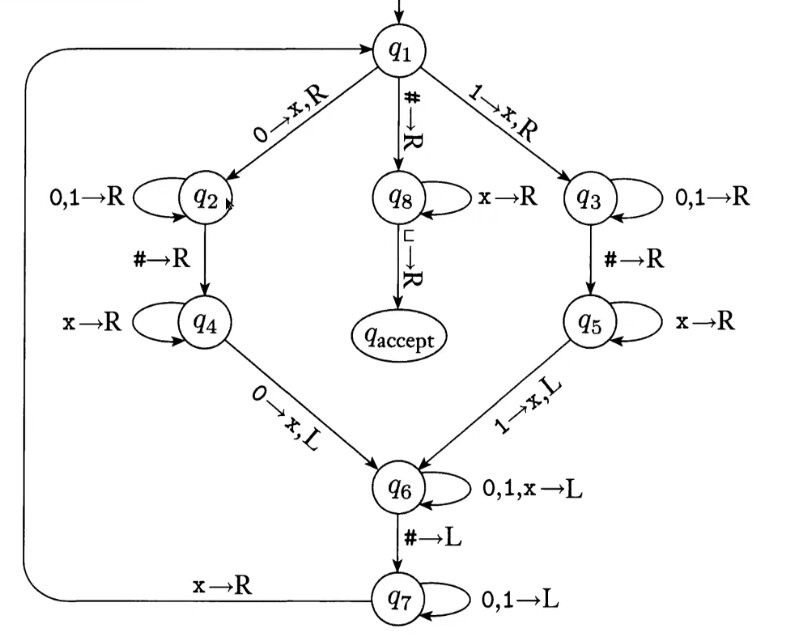
\includegraphics[width=.9\linewidth]{../media/img/grafoEs1.jpg}
\end{center}
\paragraph{Stringa di 0 di lunghezza 2\textsuperscript{n}}
\label{sec:org7904beb}
\begin{center}
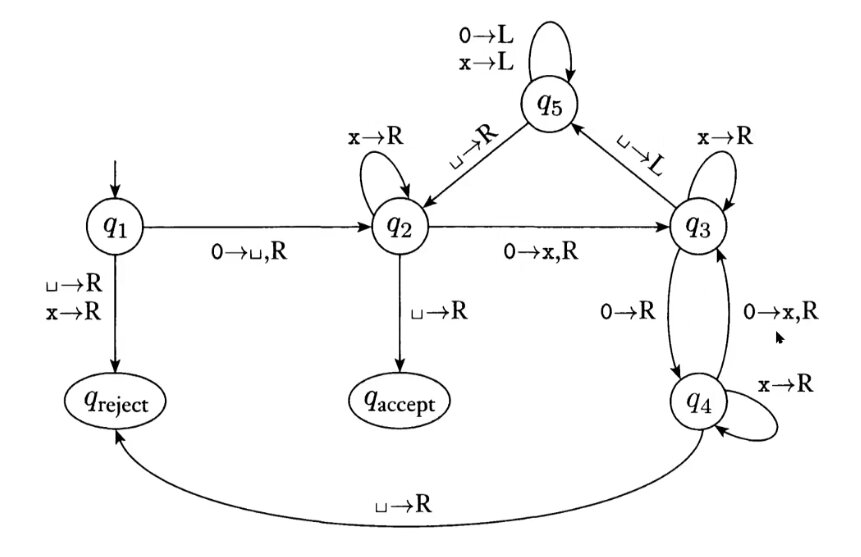
\includegraphics[width=.9\linewidth]{../media/img/graphPowerOfTwoLength.jpg}
\end{center}
\subsubsection{Macchine Turing a piú registri}
\label{sec:org5316a7a}
Con piú \emph{tapes} diventa molto piú semplice controllare stringhe, ci si avvicina nel comportamente ad una macchina di Von Neumann
Il primo nastro é l'Input, gli altri sono registri
\(\delta: Q \times \Gamma^{k} \longrightarrow Q \times \Gamma^{k} \times \{L,R,S\}^{k}\)
\begin{itemize}
\item con \(k\) simboli / tapes
\item \(S\) é \texttt{StayPut}
\end{itemize}

Si puó simulare una \texttt{MT} a piú nastri con una \texttt{MT} ad un nastro solo
\begin{itemize}
\item perché? per semplificare la definizione di calcolo
\item se un algoritmo a piú nastri é lineare su un nastro sará \textbf{quadratico}
\end{itemize}
\begin{center}
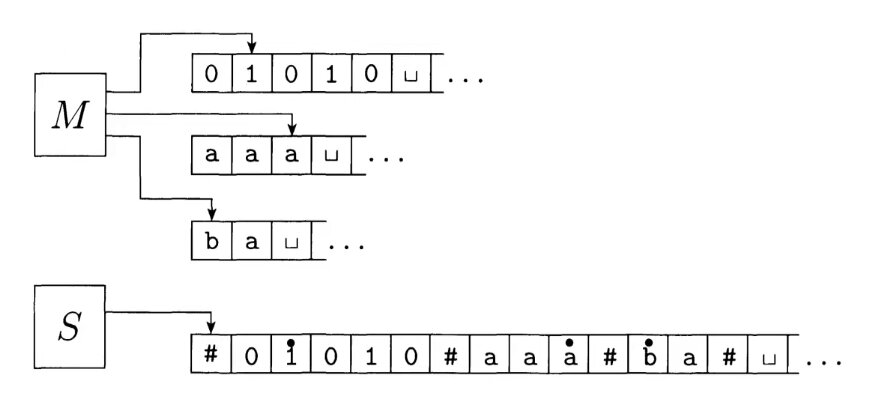
\includegraphics[width=.9\linewidth]{../media/img/3tapes1tape.jpg}
\end{center}
\subsubsection{Enumeratori}
\label{sec:org5591b4c}
Sono \texttt{TM} che enumerano stringhe.

\(\textsc{theorem}\)     Si puó definire un enumeratore \(E\) che enumeri un linguaggio \(L\) se e solo se esiste una \texttt{TM} \(M\) che riconosca (decida positivamente) il linguaggio \(L\)
\(\textsc{proof}\)      Partiamo a dimostrare che se esiste un tale \(E\) allora esiste una \(M\) che riconosca il linguaggio enumerato \(L\)

Possiamo definire \(M\) su input \(w\):
\begin{itemize}
\item simula \(E\)
\item per ogni stringa enumerata da \(E\) confrontala con \(w\)
\item se \(w\) é uguale \emph{accetta}, altrimenti continua con la simulazione di \(E\)
\end{itemize}

Da questa costruzione si evince che \(M\) accetta solo le stringhe enumerate da \(E\) e quindi nel linguaggio \(L\), \(M\) riconosce \(L\).

Ora si dimostra l'altra direzione. Se \(M\) riconosce il linguaggio \(L\) definiamo un enumeratore \(E\):
\begin{itemize}
\item ignora l'input
\item ripeti per \(i=0,1,\cdots\)
\begin{itemize}
\item esegui per \(i\) passi \(M\) su \(s_1,s_2,s_3,\cdots\)
\item se \(M\) accetta, stampa la \(s_j\) accettata
\end{itemize}
\end{itemize}

Questa macchina di turing \(E\) simula \(M\) su tutte le stringhe \(s_j\) che appartengono a \(\Sigma^*\) per \(i\) passi di simulazione, non terminando mai.
In questa simulazione sostanzialmente si simula in parallelo la macchina \(M\) su tutte le stringhe possibili in input (per un numero di passi di computazione sempre maggiore), stampando tutte e sole le \(s_j\) accettate da \(M\).
Viceversa se una stringa appartiene ad \(L\) questa viene accettata in un numero finito di passi da \(M\), e quindi dato abbastanza tempo \(E\) la stamperá. Quindi \(E\) enumera il linguaggio \(L\).

\subsection{Decidibilitá}
\label{sec:orga8ab610}
Per un \texttt{DFA} possiamo definire una \texttt{TM M} che lo simula e verifica l'accettazione o meno dell'Input
\href{../media/img/decidable-recognizable.jpg}{Decidable - Turing-recognizable}
\begin{itemize}
\item \texttt{NFA} convertibili
\item \texttt{RegEx} convertibili
\end{itemize}

\subsubsection{Definizioni}
\label{sec:orgd848f1b}
Sia \(L\) un linguaggio definito sull'alfabeto \(\Sigma\), e quindi sottoinsieme di \(\Sigma^*\)
Allora \(\forall w \in \Sigma^*\):
\begin{itemize}
\item Decidibile, esiste una \(M\) che decide \(L\)
\begin{itemize}
\item \(w\in L\): \(M\) accetta \(w\)
\item \(w\notin L\): \(M\) non accetta \(w\)
\end{itemize}
\item Positivamente Decidibile (\emph{riconoscibile})
\begin{itemize}
\item \(w \in L\): \(M\) accetta \(w\)
\item \(w \notin L\): \(M\) non accetta \(w\) o non termina
\end{itemize}
\item Negativamente Decidibile
\begin{itemize}
\item \(w \in L\): \(M\) accetta \(w\) o non termina
\item \(w \notin L\): \(M\) non accetta \(w\)
\end{itemize}
\end{itemize}

Allora definiamo \(\overline{L} = \{w\in \Sigma^* \mid w \notin M\}\) \textbf{linguaggio complemento} di \(L\)
Per i linguaggi complemento si scambiano decidibilitá positiva e decidibilitá negativa:
\begin{itemize}
\item \(L\) decidibile \(\iff\) \(\overline{L}\) decidibile
\item \(L\) positivamente decidibile \(\iff\) \(\overline{L}\) negativamente decidibile
\item \(L\) negativamente decidibile \(\iff\) \(\overline{L}\) positivamente decidibile
\end{itemize}

Esistono indebolimenti del decisore, ovvero decisori \emph{parziali}

\subsubsection{Teorema di Post}
\label{sec:org646b628}
\texttt{4.22}
Linguaggio \(L\) decidibile \(\iff\) é \uline{positivamente} e \uline{negativamente} decidibile
\begin{itemize}
\item \(M\) termina sempre \(\forall w \in \Sigma^{*}\)
\item \(M\) é un decisore che simula \(M_{1}\) e \(M_{2}\) in parallelo
\begin{itemize}
\item il primo che termina decide
\end{itemize}
\end{itemize}

Riformulando
\begin{itemize}
\item un linguaggio é decidibile esattamente quando esso e il suo complemento sono \uline{positivamente decidibili}
\end{itemize}

\(\textsc{\textbf{proof}}\)   Si dimostra prima una direzione e poi l'altra della bi-implicazione
\begin{enumerate}
\item \(\Rightarrow\)
\begin{itemize}
\item Se \(A\) é decidibile allora segue direttamente che \(A\) e \(\overline{A}\) sono positivamente decidibili
\begin{itemize}
\item per definizione di decidibilitá e complemento di un linguaggio
\end{itemize}
\end{itemize}

\item \(\Leftarrow\)
\begin{itemize}
\item Se \(A\) e \(\overline{A}\) sono positivamente decidibili, definiamo \(M_1\) e \(M_2\), decisori positivi di uno e dell'altro
\item Si definisce \(M\), decisore di \(A\)
\begin{itemize}
\item \(M =\) Su input \(w\):
\begin{enumerate}
\item Esegui \(M_1\) e \(M_2\) sull'input \(w\) in parallelo
\item Se \(M_1\) accetta, \emph{accept}; se \(M_2\) accetta, \emph{rifiuta}
\end{enumerate}
\end{itemize}
\item Ogni stringa \(w\) appartiene a \(A\) o \(\overline{A}\)
\begin{itemize}
\item Segue che per qualsiasi input una tra \(M_1\) e \(M_2\) deve accettare
\end{itemize}
\item \(M\) termina quando una tra \(M_1\) e \(M_2\) accetta
\begin{itemize}
\item Segue che \(M\) termina sempre, quindi é un decisore
\end{itemize}
\item Inoltre \(M\) accetta tutte le \(w \in A\) e rifiuta tutte le \(w \notin A\), quindi \(M\) é un decisore per \(A\)
\begin{itemize}
\item \(A\) quindi é decidibile in quanto ne esiste un decisore \(M\)                                            \(\blacksquare\)
\end{itemize}
\end{itemize}
\end{enumerate}

\subsubsection{Mapping Reducible Language}
\label{sec:org8362eae}
Il Linguaggio \(A\) é \emph{mapping reducible} al linguaggio \(B\):

\(A \le_{m}B\)

se esiste una \emph{funzione computazionale} \(f\) tale che:

\(w \in L(A) \iff f(w) \in L(B)\)

\begin{center}
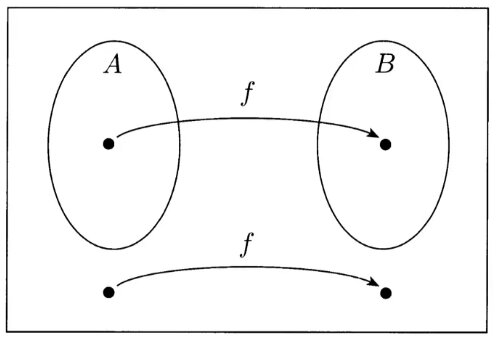
\includegraphics[width=.9\linewidth]{../media/img/mapping-reducibility.jpg}
\end{center}

Seguono i corollari:
\begin{itemize}
\item Se \(A \le_{m}B\) e \(B\) é decidibile \(\implies A\) é decidibile
\begin{itemize}
\item si dimostra costruendo la funzione e poi eseguendo \(B\) sull'input trasformato
\item stessa dimostrazione per la decidibilitá positiva
\end{itemize}
\item Se \(A \le_{m}B\) e \(A\) non é positivamente decidibile \(\implies B\) non é positivamente decidibile
\begin{itemize}
\item \(\textsc{\textbf{proof}}\)   Supponendo \(A = \overline{A_{TM}}\)
\begin{enumerate}
\item \(A \le_m B\)
\item \(\overline{A} \le_m \overline{B}\)
\item \(A_{TM} \le_m \overline{B}\)
\begin{itemize}
\item ma se \(\overline{B}\) fosse negativamente decidibile (quindi \(B\) positivamente decidibile) allora per la proprietá di cui sopra \(A_{TM}\) sarebbe negativamente decidibile
\item Ma \(A_{TM}\) non puó esserlo, altrimenti sarebbe decidibile per il Teorema di Post: contraddizione.     \(\blacksquare\)
\end{itemize}
\end{enumerate}
\end{itemize}
\end{itemize}

\subsubsection{Macchina di Turing Universale}
\label{sec:orgce5f614}
\[U = \text{"Su input }\langle M,w \rangle\text{, dove } M \text{ é una TM e } w \text{ é una stringa"} \]
\begin{enumerate}
\item Simula \(M\) su \(w\)
\item Se \(M\) accetta, \emph{accetta}; se \(M\) rifiuta, \emph{rifiuta}
\end{enumerate}

Se \(M\) cicla, \(U\) cicla di conseguenza

La macchina universale é definita a partire da \(M\) codificando in un alfabeto binario tutti i simboli di \(M\). La macchina \(U\) é definita utilizzando un alfabeto \(\Sigma=\{0,1\}\), quindi un qualsiasi stato o simbolo \(s\) di \(M\) sará convertibile in una stringa binaria \(s^*\in \Sigma^*\)
Nelle tape di \(U\) tutti i simboli sono delimitati da \#.

Queste codifiche sono utilizzate nelle 5 tape di \(U\), definite in questo modo:
\begin{enumerate}
\item la funzione di transizione \(\sigma\) di \(M\), questa tape é read-only e qui sono listate tutte le transizioni di \(M\) nella forma \(q^*, a^*,q'^*,a'^*,m^*\) dove \(a\) sono simboli di \(M\) e \(m\) sono \(L\) o \(R\)
\item lo stato corrente di \(M\), \(q^*\)
\item lo stato accettante di \(M\), \(q_{accept}^*\)
\item lo stato di rifiuto di \(M\), \(q_{reject}^*\)
\item la tape di simulazione di \(M\)
\end{enumerate}

La macchina universale procede leggendo lo stato corrente di \(M\) e il simbolo \(a^*\) che si trova sotto la testina di lettura di nella tape 5. Quindi scorre le quintuple nella prima tape, se non trova una corrispondenza rifiuta. Se trova una corrispondenza allora sovrascrive la tape 2 con il nuovo stato indicato dalla funzione di transizione e sovrascrive \(a^*\) nella tape 5 con la nuova \(a'^*\) indicata dalla transizione e aggiungendo un divisore \#. fatto questo simula il movimento a destra o a sinistra della testina di \(M\) spostandosi nella direzione indicata fino ad un \#.

\subsubsection{Problemi Decibidili}
\label{sec:orgc5d1b9c}
\(E_{\textsc{dfa}} = \{\langle A \rangle \mid A\mbox{ is a \textsc{dfa} and } L(A)=\emptyset \}\)
\begin{itemize}
\item decidibile studiando i percorsi nel grafo delle transizioni
\end{itemize}
\(EQ_{\textsc{dfa}} = \{\langle A \rangle\mid A\mbox{ is a \textsc{dfa} and } L(A)=\emptyset\}\)
\begin{itemize}
\item automa che descrive la differenza simmetrica dei linguaggi
\item si riduce a \(E_{\textsc{dfa}}\)
\end{itemize}
\(A_{\textsc{CFG}}=\{\langle G,w \rangle \mid G\mbox{ is a \textsc{CFG} that generates string }w\}\)
\begin{itemize}
\item tempo di accettazione \(2^n\)
\item non c'é problema di fermata
\end{itemize}
\(E_{\textsc{CFG}}=\{\langle G \rangle \mid G\mbox{ is a \textsc{CFG} and }L(G) = \emptyset\}\)

\subsubsection{Problemi Indecidibili}
\label{sec:orgc5f935b}
Per molti problemi si utilizza la tecnica della riduzione
\begin{itemize}
\item se un problema che sappiamo non decidibile si puó ridurre al problema che stiamo studiando allora anche questo non sará decibidile
\end{itemize}
\paragraph{Eguaglianza Chompsky}
\label{sec:org3570a29}
\(EQ_{\textsc{CFG}}=\{\langle G,H \rangle \mid G\mbox{ and }H\mbox{ are \textsc{CFG}s and }L(G) = L(H)\}\)
\paragraph{Accettazione}
\label{sec:org0f79967}
\texttt{4.11}
Problema \uline{positivamente decidibile}

\(\textsc{proof}\)   Si procede per \emph{diagonalizzazione} utilizzando due \texttt{TM} di supporto \(H\) e \(D\)

\(A_{\textsc{TM}}=\{\langle M,w \rangle \mid M\mbox{ is a \textsc{TM} and }M\mbox{ accepts }w\}\)
\begin{itemize}
\item simulabile con una macchina \(U\) di Turing universale
\begin{itemize}
\item macchina capace di simulare qualsiasi macchina utilizzando 5 tape
\end{itemize}
\item si osserva l'esecuzione che non termina
\end{itemize}
Si prova utilizzando la tecnica della \emph{diagonalizzazione} scoperta dal matematico \href{20211014120018-georg_cantor.org}{Georg Cantor} nel 1873
\begin{itemize}
\item iniezione - suriezione (biezione)
\begin{itemize}
\item corrispondenza 1 a 1
\end{itemize}
\item prova che non esiste una enumerazione per un dato insieme di numeri
\begin{itemize}
\item per i Reali si cambia nella ennesima enumerazione la ennesima cifra dopo la virgola
\begin{itemize}
\item si trova cosí un numero che differisce per una cifra da tutti i numeri enumerati
\end{itemize}
\end{itemize}
\item esistono infinite terne
\end{itemize}


\(\textsc{\textbf{proof}}\)      Si definiscono delle \texttt{MT} di supporto:

\[H(\langle M,w \rangle) = \begin{cases}
\textit{accept} \quad &\text{if }M\text{ accepts }w \\
\textit{reject} \quad &\text{if }M\text{ does not accept }w
\end{cases}\]

\begin{itemize}
\item supponiamo che \texttt{H} esista, e accetti se \texttt{M} accetta \texttt{w} e rifiuti altrimenti
\end{itemize}

\[D(\langle M \rangle) = \begin{cases}
\text{accept} \quad &\text{if }M\text{ does not accept } \langle M \rangle \\
\text{reject} \quad &\text{if }M\text{ accepts } \langle M \rangle
\end{cases}\]

\begin{itemize}
\item \texttt{D} prende in input una macchina \texttt{M} e con un decisore \texttt{H} che decide \texttt{M} con input la propria descrizione \(\langle M \rangle\), accetta se \texttt{H} rifiuta e viceversa, continua con altre macchine
\begin{itemize}
\item diagonalizza infinite macchine \texttt{M}
\end{itemize}
\end{itemize}

Allora si procede diagonalizzando con \(D\) applicato a \(\langle D\rangle\)
\[D(\langle D \rangle)\begin{cases}
\text{accept} \quad &\text{if }D\text{ does not accept }\langle D \rangle \\
\text{reject} \quad &\text{if }D\text{ accepts }\langle D \rangle
\end{cases}\]
\begin{itemize}
\item dovrebbe rifiutare se \(D\) accetta
\item dovrebbe accettare altrimenti
\begin{itemize}
\item non puó terminare perché per terminare avrebbe bisogno di dare la risposta opposta di se stesso
\end{itemize}
\end{itemize}
\uline{Abbiamo raggiunto una contraddizione}                                                             \(\blacksquare\)

\paragraph{Immortalitá}
\label{sec:org02cc6a9}
\texttt{4.23}
\(\overline A_{\textsc{tm}}\) \uline{positivamente decidibile} \(\implies  A_{\textsc{tm}}\) \uline{negativamente decidibile} per \texttt{T.Post}
\begin{itemize}
\item Falso per \texttt{4.11}
\end{itemize}
\paragraph{Fermata}
\label{sec:orgaa24ddb}
\texttt{5.1}
Il problema della decisione per \(L_{1}\) si riduce al problema della decisione per \(L_{2}\) se sappiamo trasformare un decisore per \(L_{2}\) in un decisore per \(L_{1}\)

\(\textsc{halt}_{\textsc{tm}}=\{\langle M,w\rangle \mid M \mbox{ is a \textsc{tm} and }M \mbox{ halts on input } w\}\)
\begin{itemize}
\item \(A_{\textsc{tm}} <_m \textsc{Halt}_{TM}\)
\end{itemize}

\(\textsc{\textbf{proof}}\)     Per contraddizione. Supponiamo esista una \texttt{TM} \(R\) che decida la fermata, definiamo una \texttt{TM} \(S\) che decide l'accettazione. Ma l'accettazione non é decidibile.
Definiamo \(S\) su input \(w\):
\begin{itemize}
\item Se \(R\) accetta \(\langle M,w \rangle\) procedi, altrimenti rifiuta
\item Simula \(M\) su \(w\), se accetta fa altrettanto, altrimenti rifiuta
\end{itemize}

\(A_{\text{TM}} \le_m \text{HALT}_{\text{TM}}\) in quanto se \(R\) accetta significa che \(M\) termina, accettando o rifiutando. Se diverge \(w\) non appartiene al linguaggio riconosciuto da \(M\) e \(S\) puó rifiutare.
Per ció \(S\) accetta tutte e sole le stringhe in \(L\), ovvero riconosciute da \(M\).

Ma questa é una contraddizione  in quanto si dimostra che \(A_{\text{TM}}\) non é decidibile.    \(\blacksquare\)


\paragraph{Decibidilitá dei Linguaggi di Chompsky}
\label{sec:org8879098}
\emph{Simboli, Produzioni, Terminali}
Un linguaggio definibile da una grammatica in forma normale di Chompsky é detto \texttt{context-free}
Si dimostra che il numero di passi per derivare una stringa di lunghezza \(n\) é \(2n-1\)

Questo implica che il problema é decidibile, anche se in tempo esponenziale
\begin{itemize}
\item si scrivono sulla tape 2 tutte le deduzioni di lunghezza \(2n-1\)
\item si controlla la correttezza una ad una, se ne si trova una corretta e che corrisponde accettiamo, altrimenti continuiamo, se alche l'ultima non va bene rifiutiamo
\end{itemize}
Per ridurre la complessitá si utilizza la \textbf{programmazione dinamica}
\begin{itemize}
\item ci si appunta i risultati intermedi
\end{itemize}
\paragraph{Emptyness}
\label{sec:orga8a5152}
\texttt{5.2}
Si dimostra per assurdo, se esistesse si potrebbe risolvere l'accettazione
\begin{itemize}
\item si riduce a \(A_{\textsc{tm}}\)
\begin{itemize}
\item \(A_{\textsc{tm}} <_m E_{\textsc{tm}}\)
\end{itemize}
\end{itemize}

\(\textsc{\textbf{proof}}\)   Per contraddizione. Supponiamo esista una \(R\) tale che decida la emptyness, dato una stringa di input \(w\) si modifica \(M\) per accettare solo questa stringa.
Definiamo \(M\), su input \(x\):
\begin{itemize}
\item se \(x \neq w\) rifiuta
\item altrimenti accetta
\end{itemize}

Questa macchina decide il linguaggio che contiene la sola stringa \(w\).

Allora \(S\), su input \(\langle M, w \rangle\):
\begin{itemize}
\item costruisce la \(M\) modificata come specificato
\item esegue \(R\) su \(M\), se \(R\) accetta allora rifiuta, e viceversa
\end{itemize}

In questo modo abbiamo ridotto l'accettazione alla emptyness:
\(R\) rifiuta se e solo se \(M\) accetta \(w\), e quindi il linguaggio \(L\) riconosciuto da \(M\) non é vuoto. Viceversa se \(M\) rifiuta \(w\) allora \(R\) accetterá in quanto \(L\) riconosciuta da \(M\) é il linguaggio vuoto. Quindi \(S\) decide l'accettazione. Contraddizione in quanto l'accettazione é non decidibile.              \(\blacksquare\)


\paragraph{Equality}
\label{sec:org2080172}
\texttt{5.4}
Intesa tra due \texttt{MT}
\begin{itemize}
\item se sapessi deciderla potrei decidere anche l'\texttt{Emptyness}
\begin{itemize}
\item In quanto \(E_{\text{TM}}\) é considerabile un caso particolare di \(EQ_{\text{TM}}\)
\item tra una macchiana e la macchina che rifiuta sempre
\end{itemize}
\end{itemize}

Anche per i reali:
\begin{itemize}
\item calcoli diversi portano anche arrotondamenti diversi, per questo reali rigorosamente uguali possono risultare diversi
\item \(A_{\textsc{tm}}<_m EQ_{\textsc{Real}}\)
\begin{itemize}
\item e di conseguenza anche il < e il >
\end{itemize}
\end{itemize}



\(EQ_{TM} = \{\langle M_{1}, M_{2} \rangle \mid L(M_{1}) = L(M_{2})\}\)
\(\blacksquare\)
\(\textsc{proof}\)    Si dimostra per riduzioni:
\begin{enumerate}
\item \(A_{TM} \le_{m} \overline{EQ}_{TM}\)
\begin{itemize}
\item questo indica che \(EQ_{TM}\) non puó essere negativamente decidibile
\item spostiamo al decidibilitá a \(A_{TM}\)
\end{itemize}
\item \(\overline A_{TM} \le_{m} EQ_{TM}\)
\begin{itemize}
\item questo indica che \(EQ_{TM}\) non puó essere positivamente decidibile
\end{itemize}
\end{enumerate}


Ora basta raggiungere queste conclusioni per chiudere la dimostrazione.
\begin{enumerate}
\item Definisco una macchina \(F\) che implementa la funzione \(f\) che riduce \(A\) a \(\overline{EQ}\)
\begin{itemize}
\item \(\langle M, w \rangle \rightarrow^{F} \langle M_{1}, M_{2} \rangle\)
\item se \(L(M_{1}) \neq L(M_{2})\) allora \(M\) accetta \(w\)
\begin{itemize}
\item \(M_{1}\) rifiuta sempre
\begin{itemize}
\item \(q_{0} = q_{\text{reject}}\)
\end{itemize}
\item \(M_{2}\)
\begin{itemize}
\item prende \(x\) e lo ignora
\item esegue \(M\) su \(w\) e accetta se \(M\) accetta
\begin{itemize}
\item \(\begin{cases} M \mbox{ accetta}: & L(M_{2})=\Sigma^{*}\\M \mbox{ non accetta}: & L(M_{2}) = \emptyset  \end{cases}\)
\end{itemize}
\end{itemize}
\item \(L(M_{1}) \neq L(M_{2}) \iff M \mbox{ accetta }w\)
\end{itemize}
\end{itemize}
\item Definisco una Macchina \(G\) che implementa la funzione \(g\) che riduce \(\overline A\) a \(EQ\)
\begin{itemize}
\item \(\langle M, w \rangle \rightarrow^{G} \langle M_{1}, M_{2} \rangle\)
\item se \(L(M_{1}) \neq L(M_{2})\) allora \(M\) non accetta \(w\)
\begin{itemize}
\item \(M_{1}\) accetta sempre
\begin{itemize}
\item \(q_{0} = q_{\text{accept}}\)
\end{itemize}
\item \(M_{2}\)
\begin{itemize}
\item prende \(x\) e lo ignora
\item esegue \(M\) su \(w\) e accetta se \(M\) accetta
\begin{itemize}
\item \(\begin{cases} M \mbox{ accetta}: & L(M_{2})=\Sigma^{*}\\M \mbox{ non accetta}: & L(M_{2}) = \emptyset  \end{cases}\)
\end{itemize}
\end{itemize}
\item \(L(M_{1}) \neq L(M_{2}) \iff M \mbox{ non accetta }w \qquad\qquad \blacksquare\)
\end{itemize}
\end{itemize}
\end{enumerate}

\paragraph{Corrispondenza di Post}
\label{sec:org3a852ff}
\texttt{PCP - 4.22}

\(A_{TM} \le_{m} \text{PCP}\)

Questo problema (domino) contiene la Macchina di Turing
\begin{itemize}
\item in quanto corrisponde alla visualizzazione della \hyperref[sec:org8b15e85]{Configurazione di una TM}
\begin{itemize}
\item visualizzando la storia del calcolo della macchina
\end{itemize}
\end{itemize}

Si definisce un \emph{Modified Post Correspondance Problem}:

\(A_{TM} \le_{m} \text{MPCP} \le_{m} \text{PCP}\)

Si decide che il primo elemento dell'insieme deve essere utilizzato all'inizio
\begin{itemize}
\item sopra abbiamo \(n-1\) passi di calcolo
\item sotto abbiamo \(n\) passi di calcolo
\end{itemize}
Questi \emph{domini} rappresentano le funzioni di transizione attraverso le configurazioni della \texttt{TM}
\begin{itemize}
\item \([\frac{\#qa}{\#rb}]\)
\begin{itemize}
\item \(\delta(q,a) = (r,b,L)\)
\end{itemize}
\item compresi i pezzi dei singoli simboli, che si mantengono da un istante all'altro se non toccati dalla trasformazione di stato
\begin{itemize}
\item \([\frac{1}{1}]\)
\item \([\frac{0}{0}]\)
\item \([\frac{\sqcup}{\sqcup}]\)
\item \([\frac{\#}{\sqcup\#}]\)
\begin{itemize}
\item utilizzato quando lo stato deve spostarsi a destra oltre l'ultimo simbolo
\end{itemize}
\end{itemize}
\end{itemize}

Si devono definire dei domino per l'accettazione, che faccia \emph{match}:
\([\frac{q_{accept}\#\#}{\qquad \;\;\;\: \#}]\)
Per arrivare a questo \emph{accept}:
\(\forall a\in \Gamma\)
\begin{itemize}
\item \([\frac{a\: q_{accept}}{\quad q_{accept}}]\)
\item \([\frac{q_{accept} \: a}{q_{accept}\quad}]\)
\end{itemize}
\paragraph{Tassellazione - Wang Tiles}
\label{sec:org01c92a6}
\href{https://en.wikipedia.org/wiki/Wang\_tile}{Wikipedia}
Solo negativamente decidibile
\begin{itemize}
\item le tassellazioni aperiodiche sono utilizzate per la sintesi procedurale di texture, heightfields
\end{itemize}

Si dimostra che \(\textsc{Wang}\) non é positivamente decidibile in quanto
\begin{itemize}
\item \(\overline{\textsc{Halt}} \le_m \textsc{Wang}\)
\item procedendo in maniera non deterministica, il caso di \emph{non-rifiuto} indica che un albero della computazione ha per caso scelto la configurazione corretta per risolvere il problema della tassellazione
\item la computazione non deterministica si ferma solo in caso di rifiuto di tutti i rami non deterministici, quindi se la computazione non si ferma si dovrebbe accettare
\end{itemize}

\paragraph{Esistenza di un DFA equivalente}
\label{sec:org8318c62}
\texttt{5.3}
\(A_{\textsc{tm}} <_m\textsc{Regular}_{\textsc{tm}}\)
\subsubsection{Configurazione di una TM}
\label{sec:org8b15e85}
\begin{figure}[htbp]
\centering
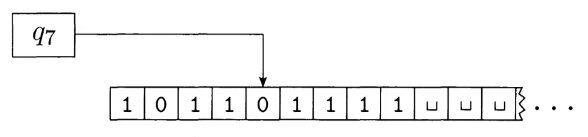
\includegraphics[width=.9\linewidth]{../media/img/tm-configuration.jpg}
\caption{configurazione di \(1011 q_{7} 01111\)}
\end{figure}
\subsubsection{Recap}
\label{sec:orgc905b87}
\begin{center}
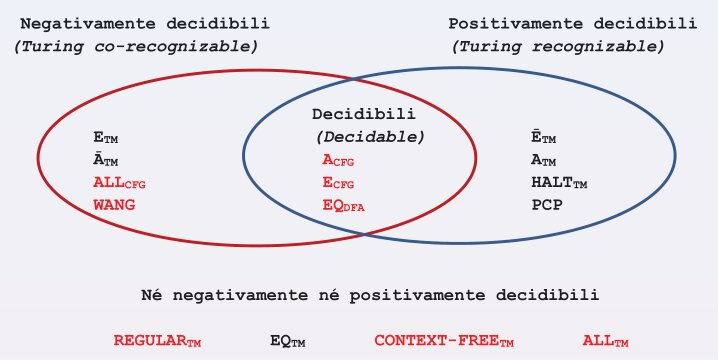
\includegraphics[width=.9\linewidth]{../media/img/decidability.jpg}
\end{center}

\begin{itemize}
\item Negativamente Decidibili
\begin{itemize}
\item \(E_{\textsc{tm}}\)
\item \(\overline A_{\textsc{tm}}\)
\item \(\textsc{All}_{\textsc{cfg}}\)
\item \(\textsc{Wang}\)
\end{itemize}
\item Decidibili
\begin{itemize}
\item \(E_{\textsc{cfg}}\)
\item \(A_{\textsc{cfg}}\)
\item \(\textsc{Eq}_{\textsc{dfa}}\)
\end{itemize}
\item Positivamente Decidibili
\begin{itemize}
\item \(\overline E_{\textsc{tm}}\)
\item \(A_{\textsc{tm}}\)
\item \(\textsc{Halt}_{\textsc{tm}}\)
\item \(\textsc{pcp}\)
\begin{itemize}
\item \hyperref[sec:org3a852ff]{Corrispondenza di Post}
\end{itemize}
\end{itemize}
\item Né negativamente né positivamente decidibili
\begin{itemize}
\item \(\textsc{Regular}_{\textsc{tm}}\)
\item \(\textsc{Eq}_{\textsc{tm}}\)
\item \(\textsc{Context-Free}_{\textsc{tm}}\)
\item \(\textsc{All}_{\textsc{tm}}\)
\begin{itemize}
\item se un programma accetta sempre
\end{itemize}
\end{itemize}
\end{itemize}
\subsection{Complessitá Temporale}
\label{sec:org08ab2e4}
Trattata nel corso di Algoritmi: \href{20210414192358-problems_algorithms.org}{Complessitá di un algoritmo}
Per lo studio della complessitá consideriamo la \uline{Macchina di Turing} (1 registro)
\begin{itemize}
\item questo in quanto la complessitá varia anche in base all'architettura
\end{itemize}

Il tempo di calcolo della macchina \(M\) é definito come

\(f : \mathbb{N} \to \mathbb{N}\) dove \(f(n)\) é il numero massimo di passi compiuti dalla macchina \(M\)

Si utilizza la \emph{notazione asintotica} o \textbf{big-O Notation}
\begin{itemize}
\item \href{20210414192358-problems_algorithms.org}{O-grande}
\end{itemize}

\[\textsc{Time}= \{L \mid L \text{ risolvibile da =TM= deterministica in }O(f(n)) \text{ polinomiale}\}\]
\[\textsc{NTime}= \{L \mid L \text{ risolvibile da =TM= non deterministica in }O(f(n))\text{ polinomiale} \}\]

Generalmente:
\begin{itemize}
\item \(\text{P} =\) classe dei linguaggi la cui appartenenza puó essere decisa velocemente
\item \(\text{NP} =\) classe dei linguaggi la cui appartenenza puó essere verificata velocemente
\end{itemize}

Non si é riuscita a provare l'esistenza di un singolo linguaggio \(\text{NP}\) che non sia in \(\text{P}\)

Piú grande problema aperto: \(\text{P}=\text{NP}\)
\begin{center}
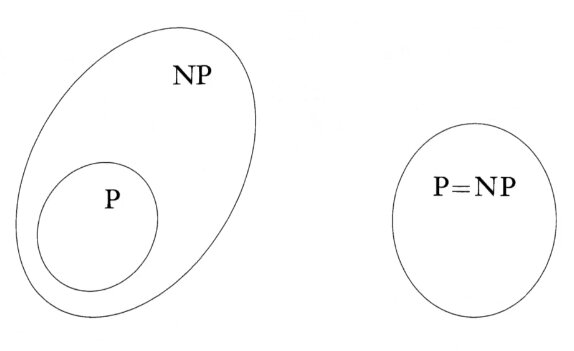
\includegraphics[width=.9\linewidth]{../media/img/P-NP.jpg}
\end{center}

\subsubsection{P}
\label{sec:org294b6b5}
Teorema \texttt{7.8}
Sia \(t(n)\) una funzione t.c. \(t(n) \ge n \implies\) qualsiasi macchina \emph{multitape} \(M\) con  tempo \(t(n)\) ha un equivalente \(O(t^2(n))\) in una macchina \(M'\) \emph{singletape}
\begin{itemize}
\item chiaro riprendendo la simulazione di \emph{multitape} in \emph{singletape}
\item un passo della simulazione \emph{singletape} impiega al massimo \(O(t(n))\) passi
\end{itemize}

La classe di tempo \textbf{Polinomiale} é definito come

\[\text{P} = \bigcup_k \textsc{time}(n^k)\]

\subsubsection{Non Determinismo}
\label{sec:org5992974}
Teorema \texttt{7.11}
Sia \(t(n)\) una funzione dove \(t(n)>n\).
Allora ogni \texttt{TM} \emph{singletape} \uline{non deterministica} con complessitá temporale \(t(n)\) ha una equivalente \texttt{TM} \uline{determinitistica} \(2^{O(t(n))}\), nel caso di una macchina multiregistro
Per una \texttt{TM} deterministica a registro singolo si avrá sempre complessitá \(2^{O(t(n))}^2 = 2^{O(t(n))}\)

L'esplorazione dell'albero non deterministico é svolto utilizzando \emph{l'ordine lessicografico}
\begin{itemize}
\item in profonditá
\item questo é posto nell'\emph{address tape} della macchina \textbf{deterministica} corrispondente
\item a livello \(n\) l'albero ha massimo \(k^{n}\) nodi con \(k\) numero di possibili figli
\item il numero di passi necessari all'esplorazione dell'albero é \(2^{O(m)}\)
\begin{itemize}
\item \(m\) profonditá dell'albero
\end{itemize}
\end{itemize}
\paragraph{Raggiungibilitá}
\label{sec:orgeaa4b1a}
\(\textsc{Path} = \{ \langle G,s,t  \rangle \mid G \text{ é  diretto con un cammino da }s \text{ a } t \}\)
La soluzione banale non deterministica ha \(2^{O(t(n))}\) \uline{esponenziale}

Con un algoritmo marcando i nodi man mano che vengono scoperti si raggiunge complessitá \uline{polinomiale}
\begin{itemize}
\item rappresentando il grafo con liste di adiacenza la si puó stimare \(O(n)\) nel numero di archi
\end{itemize}
\paragraph{Algoritmo di Euclide}
\label{sec:org7e9c442}
\(\textsc{RelPrime}\), il \texttt{MCD} tra due numeri Relativamente Primi é 1
\(\textsc{mcd}(x,y) = \textsc{mcd}(x \mod(y), y)\)
quindi procediamo:
\((x,y) \to (x \mod{y}, y) \to (y, x\mod{y})\to \cdots \to (x,0)\)
\(\textsc{mcd}(x,0) = x\)

I passi sono eseguiti \(min(2 \log_{2} x, 2\log_{2} y)\) ovvero proporzionali al numero di cifre nella rappresentazione binaria: \(O(n)\) quindi \uline{polinomiale}

\paragraph{Grammatiche di Chompsky}
\label{sec:org68dd727}
Per migliorare la complessitá si cerca di derivare tutte le sottostringhe di lunghezza crescente della stringa di input
\begin{itemize}
\item si memorizzano le soluzioni delle sottostringhe
\begin{itemize}
\item per ogni sottostringa la si divide in sottostringhe e si guarda la soluzione delle sottostringhe
\item in una rappresentazione matriciale la soluzione si trova nella riga precedente
\end{itemize}
\item ogni controllo richiede \(O(1)\) in quanto le sottostringhe sono sempre riconducibile ai siboli terminali
\end{itemize}
Con questo algoritmo si raggiunge \(O(n^3)\)

\subsubsection{NP}
\label{sec:org244e6b6}
Un linguaggio é \texttt{NP} \(\iff\) é deciso da un algoritmo \uline{non deterministico polinomiale}
Un \(M: O(n^k)\) \texttt{NTM} equivale a \(M': 2^{O(n^k)}\) \texttt{TM}
\begin{itemize}
\item da tempo polinomiale a tempo esponenziale
\end{itemize}

\[\text{NP} = \bigcup_k \textsc{ntime}(n^k)\]

Un linguaggio é \texttt{NP} se dispone di un \emph{verificatore} in tempo polinomiale, detto allora \emph{polinomialmente verificabile}

\textbf{Def} \texttt{7.18}
Un \textbf{verificatore} é una macchina di turing \(V\) tale che per un linguaggio \(A\):
\begin{itemize}
\item \(A = \{w \mid V \text{ accepts } \langle w,c \rangle \text{ for some string }c\}\)
\begin{itemize}
\item \(w\) riguarda i dati del problema
\item \(c\) riguarda le istruzioni della \texttt{TM}, un candidato di soluzione o almeno ci é legato in qualche maniera
\begin{itemize}
\item potrebbe essere anche il cammino della macchina non deterministica
\item la \emph{address tape} nella simulazione deterministica di una macchina non deterministica
\end{itemize}
\end{itemize}
\item si misura il tempo di un verificatore solo in funzione della lunghezza di \(w\)
\begin{itemize}
\item un verificatore polinomiale esegue in tempo polinomiale secondo la lunghezza di \(w\)
\end{itemize}
\end{itemize}

\textbf{Prova} \texttt{7.20}
Il determinismo con certificato \(c\) utilizzando \(V\) é convertito in non determinismo trovando il \(c\) in maniera non deterministica di lunghezza massima \(n^k\) (dove questo é il polinomio di complessitá)

Si dimostra quindi che le due definizioni sono equivalenti in quanto é sempre possibile convertire un \(V\) polinomiale in una \(M\) polinomiale non deterministica e viceversa.

\paragraph{NP-completo}
\label{sec:orgddcb8c4}
\(\textsc{\textbf{definition}}\)  Un linguaggio \(B\) é \(\textsc{NP}\text{-completo}\) se soddisfa le seguenti condizioni:
\begin{enumerate}
\item \(B \in \textsc{NP}\)
\item \(\forall A\in \textsc{NP}, A  <_P B\)
\begin{itemize}
\item \(A\) si riduce in tempo polinomiale a \(B\)
\end{itemize}
\end{enumerate}

Ci sono quindi due possibilitá che si escludono l'un l'altra:
\begin{itemize}
\item \(\text{P} = \text{NP}\)
\item Tutti i problemi \(\text{NP-completi}\) non sono polinomiali
\end{itemize}

La classe \(\text{NP-completo}\) descrive i problemi piú difficili in \(\text{NP}\)

\paragraph{Teorema di Cook-Levin}
\label{sec:orgc582683}
Problemi in \(\textsc{NP}\) la cui complessitá é legata a quella dell'intera classe sono detti \(\textsc{NP}\text{-completi}\)
Il problema della soddisfatibilitá (\emph{satisfiability problem}) fa parte di questa classe
\begin{itemize}
\item Una formula booleana é soddisfacibile se qualche assegnamento di 0 e di 1 fa si che la formula risulti 1
\item \(\textsc{SAT}=\{ \langle \phi \mid \phi \rangle\) é una formula booleana soddisfacibile \(\}\)
\end{itemize}

\texttt{7.27}
\(\textsc{\textbf{theorem}}\)  \(\textsc{SAT}\in \textsc{P} \iff \textsc{P}=\textsc{NP}\)

Questo teorema é implicato da \texttt{7.37}:
\(\textsc{\textbf{theorem}}\)  \(\textsc{SAT}\) é \(\textsc{NP}\text{-completo}\)
\(\textsc{\textbf{corollary}}\)   \(\text{3SAT}\) é \(\text{NP-completo}\)
\begin{itemize}
\item \(\text{CNF-SAT} \le_P \text{3-SAT}\le_P \text{CLIQUE}\)
\end{itemize}


\textbf{NB} - Per provare la \(\text{NP-completessa}\) si procede da \(\text{SAT}\) al problema in particolare


\paragraph{Hamilton's Path}
\label{sec:orgb13c0c2}
Percorso che percorre tutti il grafo a partire da \(p\) arrivando in \(t\) senza ripetizioni.
Si percorre il grafo non deterministicamente
\begin{itemize}
\item si scartano tutti i rami in cui il primo nodo non é \(p\) o \(t\) non é l'ultimo
\item si scartano i rami in cui ci sono ripetizioni
\end{itemize}

Non conosciuto algoritmo in \(\text{P}\)

\(\text{3SAT}  \le_P \textsc{HamPath}\)

\paragraph{Compositeness}
\label{sec:org2f717b0}
\(\textsc{Composites} = \{x \mid x = pq \text{ for integers }p,q > 1\}\)
Un numero composto é un numero non primo.
Esiste un algoritmo polinomiale per verificare se un numero é composto o meno ma non per trovare la sua scomposizione (o almeno non lo si é trovato)
Quindi: \(\textsc{Composites} \in \text{NP} \land \textsc{Composites} \in \text{P}\)

\paragraph{Clique}
\label{sec:orgd0bc64d}
\texttt{7.32}
Grafo \uline{non orientato}, fornito un \(k\)
\begin{itemize}
\item si richiede un \uline{sottografo} in cui 2 qualunque nodi distinti sono connessi di un arco
\end{itemize}
Non si sa se esistono algoritmi polinomiali \(\text{P}\)

\(\textsc{Clique} = \{\langle G,k \rangle \mid G \text{ is an undirected graph with a k-clique}\}\)

É \(\text{NP-completo}\)

\(\textsc{\textbf{proof}}\)   Data \(\phi\) una formula con \(k\) clausole del tipo
\begin{itemize}
\item \(\phi = (a_1 \lor b_1 \lor c_1) \land \cdots \land (a_k \lor b_k \lor c_k)\)
\end{itemize}
Si definisce la riduzione \(f\) per cui \(\textsc{Clique} <_P \text{3SAT}\)
\begin{itemize}
\item \(f\) genera la stringa \(\langle G,k \rangle\), dove \(G\) é un grafo non orientato
\item i nodi di \(G\) sono raggruppati in \(k\) triplette \(t_1,\ldots ,t_k\)
\item gli archi di \(G\) connettono tutti i nodi tranne:
\begin{enumerate}
\item nodi della stessa tripletta
\item due nodi contraddittori, come \(x_1\) e \(\overline{x_1}\)
\end{enumerate}
\end{itemize}

Si dimostra che \(\phi \in \text{3SAT} \iff G\in k\textsc{-Clique}\)
Quindi \(\text{3SAT} <_P \textsc{Clique}\)                                         \(\blacksquare\)

\paragraph{Subset-Sum}
\label{sec:orgb4fe5b2}
\texttt{7.56}
\(\textsc{Subset-Sum} = \{\langle S,t  \rangle \mid S = \{s_1,\ldots ,s_n\}\) dove esistono \(\{y_1,\ldots,y_m\}\subseteq S\) tali che \(\sum y_i  = t\}\)

Si dimostra facilmente che questo é \(\textsc{np}\) definendone un verificatore polinomiale oppure una \texttt{TM} non deterministica polinomiale che lo definisca.

\(\textsc{Subset-Sum}\) é \(\text{NP-completo}\)

La prova procede per riduzione polinomiale da \(\text{3SAT}\) a \(\textsc{Subset-Sum}\), convertendo elementi e strutture del problema che rappresentano variabili e clausole booleane.
\subsection{Complessitá Spaziale}
\label{sec:org104664c}
\texttt{8.1}
\(\textsc{\textbf{definition}}\)  Data la \texttt{TM} \(M\) che termina sempre. Si dice \emph{complessitá spaziale} di \(M\) la funzione
\(f: N\to N\), dove \(f(n)\) é il massimo numero di celle di nastro che la \(M\) passa su un qualsiasi input di lunghezza \(n\)
\subsubsection{Classi}
\label{sec:org06e2d51}
\texttt{8.2}
\(\textsc{\textbf{definition}}\)  Data \(f: N\to R^+\). Le \emph{classi di complessitá spaziale} \(\textsc{space}(f(n))\) e \(\textsc{nspace}(f(n))\), sono definiti come:
\begin{itemize}
\item \(\textsc{space}(f(n)) = \{L\mid L\) é decidibile da una TM deterministica in spazio \(O(f(n))\}\)
\item \(\textsc{nspace}(f(n)) = \{L\mid L\) é decidibile da una TM non deterministica in spazio \(O(f(n))\}\)
\end{itemize}

\(\textsc{\textbf{definition}}\)  \(\textsc{pspace}\) é la classe di linguaggi che sono decidibili in spazio polinomiale da una \texttt{TM} deterministica
\begin{itemize}
\item \[\textsc{pspace}=\bigcup_k\textsc{space}(n^k)\]
\end{itemize}
Da \texttt{8.5} segue che \(\textsc{pspace} = \textsc{npspace}\)


In sommario:
\begin{itemize}
\item \(\textsc{p} \subseteq\textsc{np} \subseteq\textsc{pspace} =\textsc{npspace} \subseteq \textsc{exptime}\)
\end{itemize}

Questo perché:
\begin{itemize}
\item \(\textsc{np} \subseteq \textsc{npspace}\) in quanto una macchina in \(f(n)\) passi puó esplorare al massimo \(f(n)\) celle di memoria
\item \(\textsc{pspace}\subseteq\textsc{exptime}\), una machina in \(\textsc{pspace}\) puó eseguire passi senza ripetersi al massimo
\begin{itemize}
\item \[f(n)\cdot 2^{O(f(n))} = \bigcup_k \textsc{time}(2^{n^k)\], dopo di che é in loop
\end{itemize}
\end{itemize}

\begin{center}
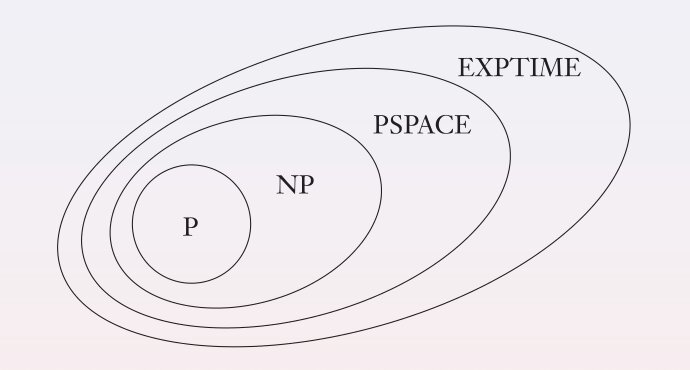
\includegraphics[width=.9\linewidth]{../media/img/complexity-classes.jpg}
\end{center}
Qualsiasi di queste inclusioni potrebbero essere eguaglianze, ma non sono state trovate prove a riguardo.

Inoltre si definiscono le classi sottolineari:
\[\textsc{L} = \bigcup_k \textsc{space}(\log n) \]
\[\textsc{NL} = \bigcup_k \textsc{nspace}(\log n) \]

E si dimostra:
\(\textsc{l} \subseteq\textsc{nl} \subseteq \textsc{p} \subseteq\textsc{np} \subseteq\textsc{pspace} =\textsc{npspace} \subseteq \textsc{exptime}\)

\subsubsection{Teorema di Savitch}
\label{sec:org29eab82}
\texttt{8.5}
Per qualsiasi funzione \(f: N \to R^+\), dove \(f(n) \ge n\),
\begin{itemize}
\item \(\textsc{nspace}(f(n))\subseteq \textsc{space}(f^2(n))\)
\end{itemize}

Il passaggio da non determinismo a determinismo per il tempo é piú impegnativo che per lo spazio, lo spazio é piú potente in quanto puó essere riutilizzato, al contrario del tempo.
\begin{itemize}
\item l'equivalente deterministico di una macchina non deterministica polinomiale ha:
\begin{itemize}
\item Tempo \(2^{O(n^k)}\)
\item Spazio \(O(n^2)\)
\end{itemize}
\end{itemize}

Da questo teorema segue che \(\textsc{PSPACE} =  \textsc{NPSPACE}\) in quanto il quadrato di un polinomiale é ancora polinomiale.
\subsubsection{GG}
\label{sec:org3bbd9c9}
Gioco Generalizzato della Geografia
\begin{itemize}
\item il gioco consiste nel spostarsi in un grafo i cui nodi sono nomi di cittá
\item gli archi vanno da un cittá il cui nome finisce con una certa lettere a un nodo/cittá che inizia per data lettera
\item ci sono due giocatori che partono da una data cittá
\item a turno scelgono un arco da percorrere, perde chi non puó scegliere un arco entrante in un nodo giá visitato
\end{itemize}

Si dimostra che \(\textsc{gg}\) é \(\textsc{pspace}\) definendo una funzione ricorsiva detta di Von Neumann \(\text{VonN}(a,X,g)\) una volta fissato il grafo \(G\)
\begin{itemize}
\item vero se esiste una strategia vincente a partire da \(a\) per il giocatore \(g\), che porta quindi ad una configurazione in cui non esiste una mossa \(b\) per il giocatore \(\lnot g\) che non violi le regole
\end{itemize}

Altro risultato della teoria é che \(\textsc{gg}\) é \(\textsc{pspace}\text{-completo}\), quindi se si scoprisse un algoritmo in tempo polinomiale che risolva \(\textsc{gg}\) questo dimostrerebbe che:
\begin{itemize}
\item \(\textsc{P = NP = PSPACE = NPSPACE}\).
\end{itemize}

In quanto per il teorema di \texttt{Savitch} \(\textsc{NPSPACE = PSPACE}\).

Questa ipotesi é ritenuta improbabile, anche se non si puó escludere.
\end{document}
